\section{Laborationsloggbok}

I figur \ref{bil:loggbok} kan laborationsloggboken som fördes vid laborationstillfället 2023-09-23 ses.

\begin{figure}[H] 
    \centering
    \begin{subfigure}{.5\textwidth}
      \centering
      \frame{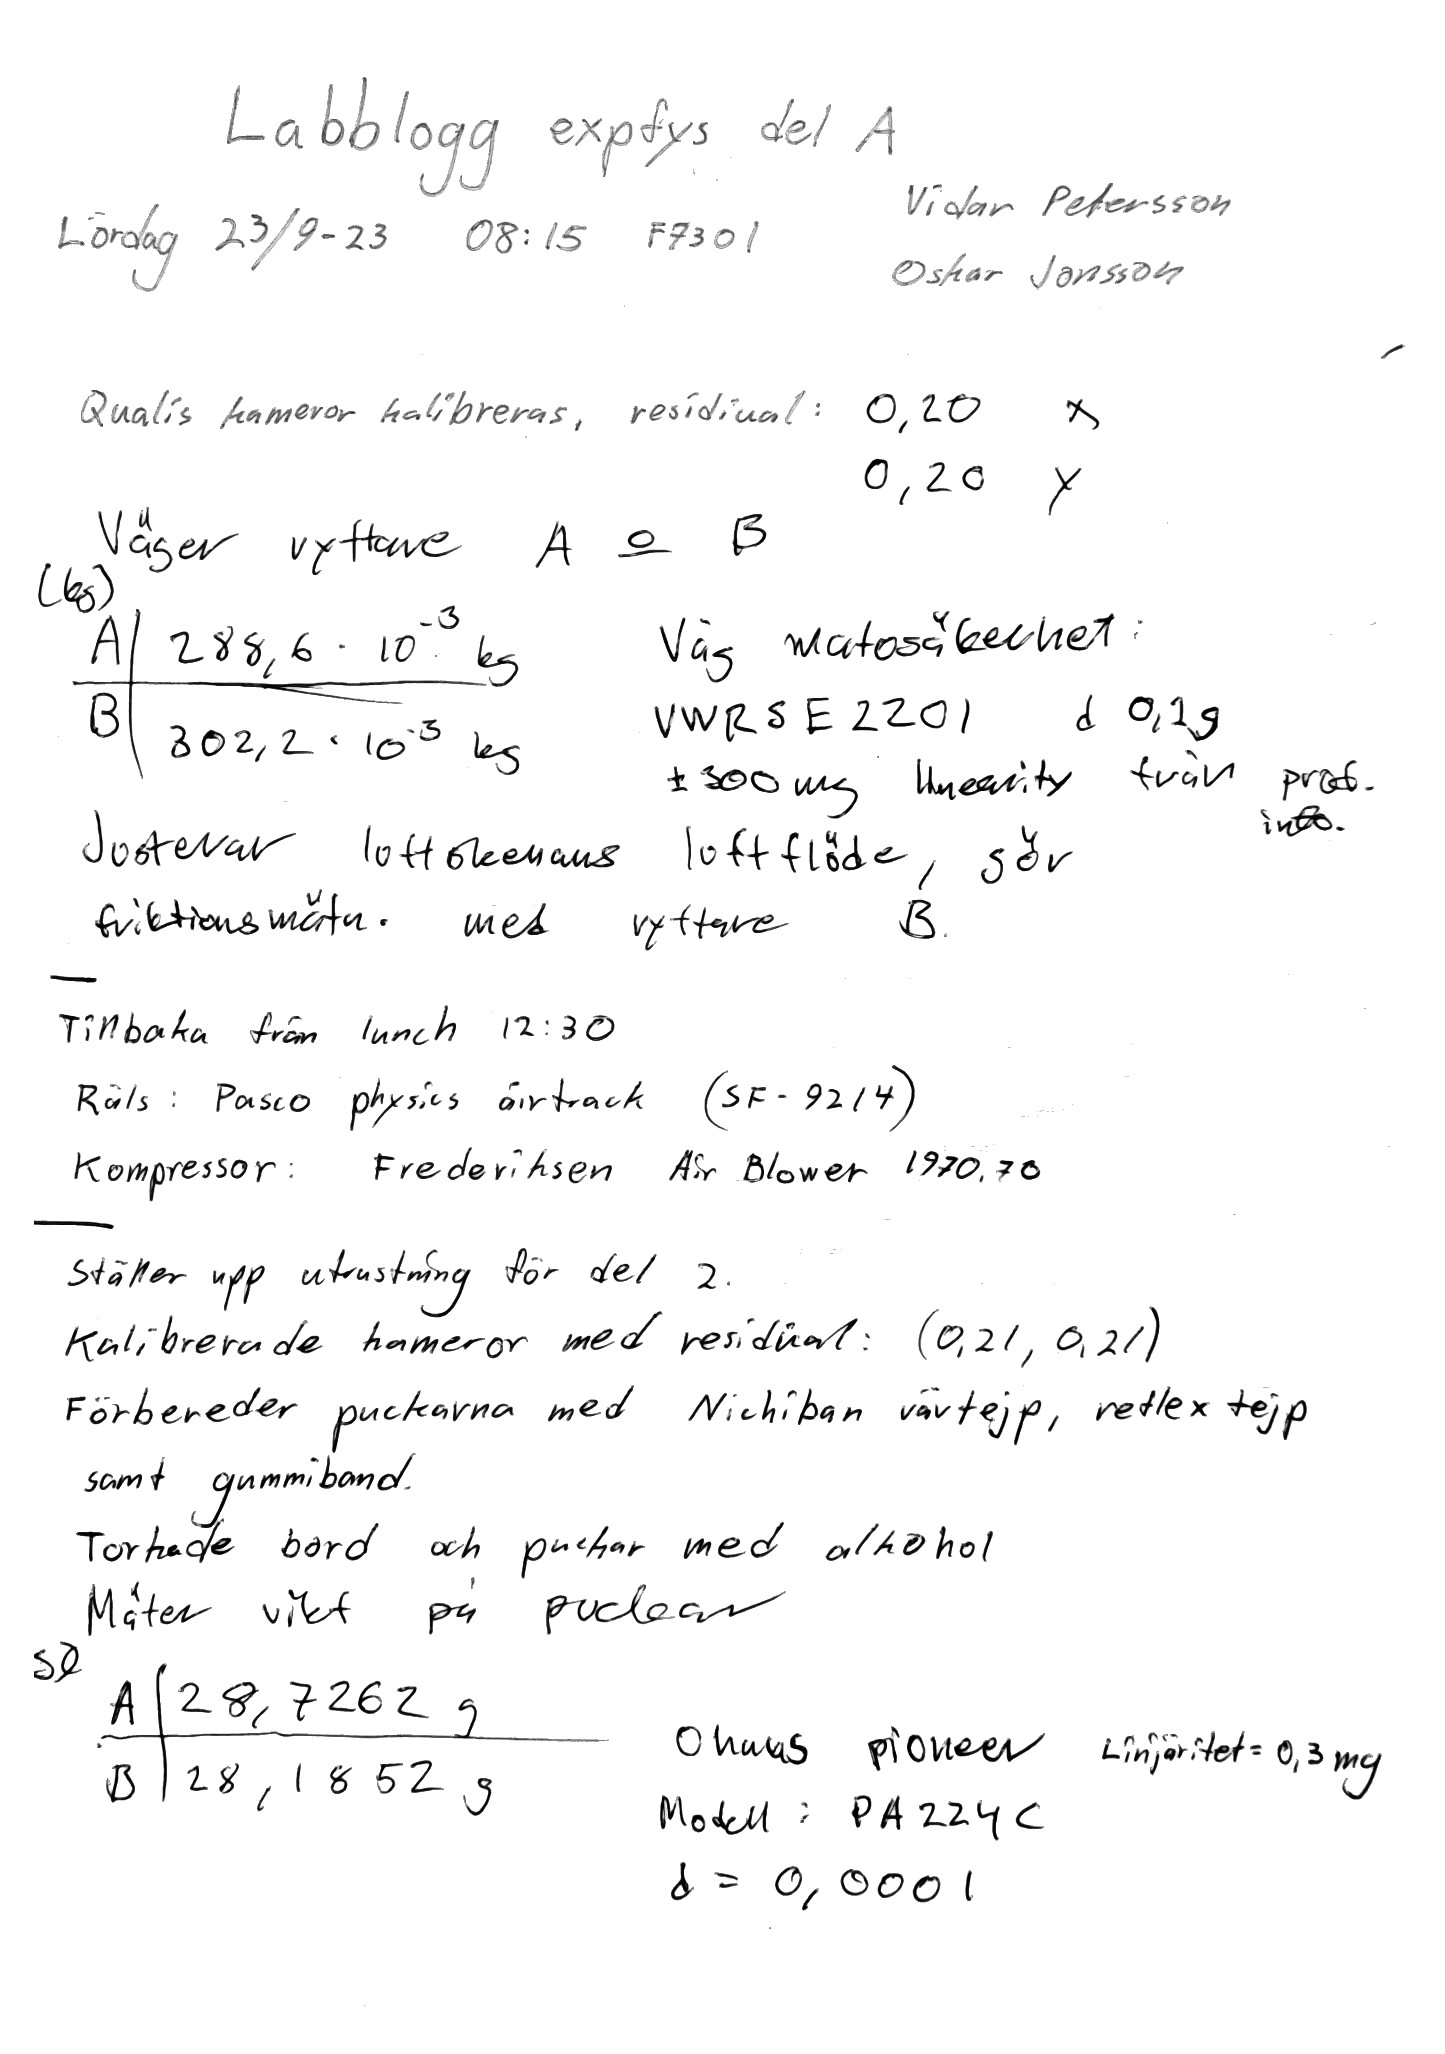
\includegraphics[width=0.85\linewidth]{bilagor/loggbok1.jpg}}
    \end{subfigure}%
    \begin{subfigure}{.5\textwidth}
      \centering
      \frame{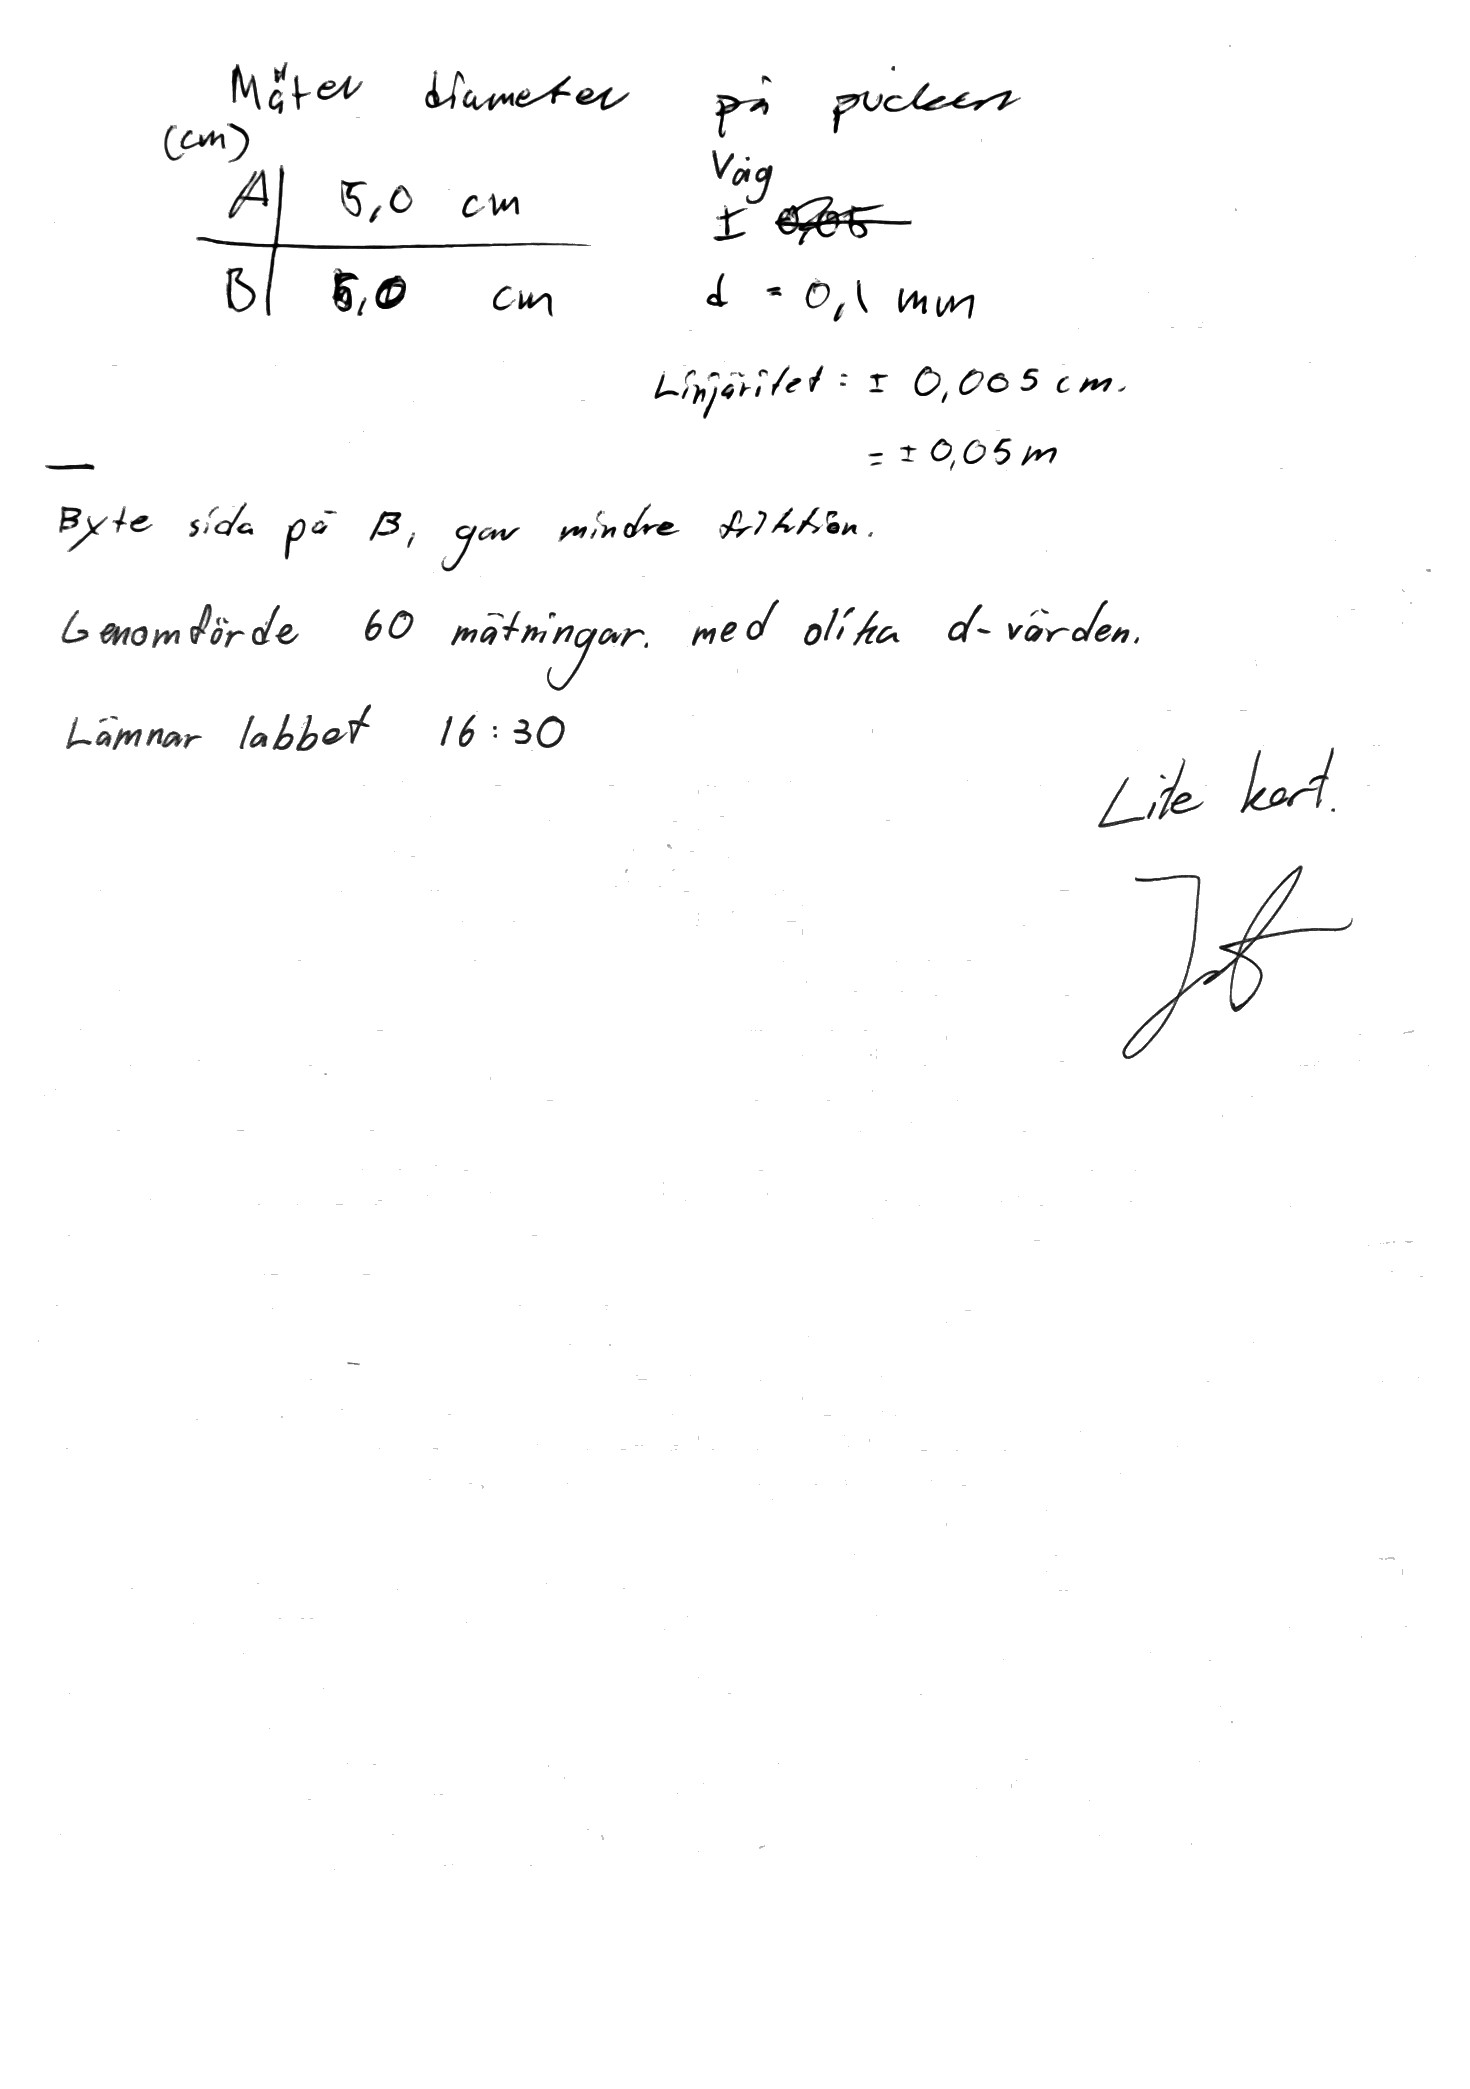
\includegraphics[width=0.85\linewidth]{bilagor/loggbok2.jpg}}
    \end{subfigure}
    \caption{Laborationsloggbok signerat av handledare.}
    \label{bil:loggbok}
\end{figure}

\section{Dataanalys}\label{bil:kod}
Denna bilaga presenterar den kod som ligger till grund för dataanalysen i arbetet. Koden använd för del 1 presenteras i lisitng \ref{lst:1main} och för del 2 i listing \ref{lst:2center_calc} och \ref{lst:2_analisys}.

\definecolor{dgray}{gray}{0.35}
\definecolor{lgray}{gray}{0.97}
\lstset{
    language=Python,
    backgroundcolor=\color{lgray},
    basicstyle=\footnotesize\ttfamily,
    commentstyle=\footnotesize\ttfamily\itshape\color{dgray},
    numberstyle=\footnotesize\ttfamily,
    numbers=left,
    frame=none,
    stepnumber=1,
    showstringspaces=false,
    tabsize=2,
    breaklines=true,
    breakatwhitespace=true,
    postbreak=\mbox{{$\hookrightarrow$}\space}
}

\lstinputlisting[
caption={Kod för dataanalys av del 1. Kod för generering av figurer har uteslutits.},
label={lst:1main},
language=Python,
]{bilagor/1_main.py}

\newpage
\lstinputlisting[
caption={Kod för numerisk beräkning av dels vilken puck mätpunkterna tillhörde och dels beräkning av masscentrums translation och rotation utifrån mätpunkternas rotation och translation i del 2.},
label={lst:2center_calc},
language=Python,
]{bilagor/2_center_calc.py}

\newpage
\lstinputlisting[
caption={Kod för numerisk beräkning av puckarnas tillstånd innan och efter kollision. Kod för generering av figurer har uteslutits.},
label={lst:2_analisys},
language=Python,
]{bilagor/2_analisys.py}


\section{Mätvärden} \label{bil:mätning}

\begin{table}[H]
\centering
\caption{Uppmätta konstanter av ryttarna i del 1.}
\label{tab:prop1}
\begin{tabular}{@{}ll@{}}
\toprule
Objekt    & Massa                                 \\ \midrule
Ryttare A  & $\SI{0.2886(1)}{kg}$                 \\
Ryttare B med gummiband& $\qty{0.3022(1)}{kg}$  \\
Ryttare B utan gummiband& $\qty{0.2982(1)}{kg}$ \\ \bottomrule
\end{tabular}
\end{table}

\begin{table}[H]
\centering
\caption{Uppmätta och beräknade konstanter av puckarna 2.}
\label{tab:prop2}
\begin{tabular}{@{}lll@{}}
\toprule
Objekt    & Massa                   & Radie             \\ \midrule
Puck A    & $\qty{0.0287262(1)}{kg}$   & $\qty{0.025(0.0005)}{m}$          \\
Puck B    & $\qty{0.0281852(1)}{kg}$   & $\qty{0.025(0.0005)}{m}$          \\ \bottomrule
\end{tabular}
\end{table}

\section{Mätutrustning} \label{bil:mätutr.}
\begin{table}[H]
\centering
\caption{Översikt över den mätutrustning som användes för att mäta objekten.}
\label{tab:mätutr.}
\begin{tabular}{@{}lllll@{}}
\toprule
Instrumenttyp & Modellnamn     & Mätte         & Upplösning        & Linjäritet            \\ \midrule
Våg           & VWR   & Ryttarna & $\SI{e-4}{kg}$    & $\SI{\pm 3e-4}{kg}$   \\
& (SE2201)   & &     &    \\
Våg           & Ohaus Pioneer & Puckarna    & $\SI{e-7}{kg}$    & $\qty{\pm 3e-7}{kg}$  \\
           & (PA224C) & &  &   \\
Skjutmått     & Okänd         & Puckarna    & $\qty{5e-5}{m}$   & -                     \\ 
Motion capture & Qualisys Oqus 300 & Alla           & $\qty{e-6}{m}$    & -                     \\ \bottomrule
\end{tabular}
\end{table}

\section{Mätosäkerhet}\label{bil:mätos}
För storheterna i figurerna beräknas i denna bilaga deras mätosäkerhet med hjälp av insamlade värden på mätutrustning samt medelvärdet av samtlig insamlad data för att få fram felfortplanAtningen för varje enskild storhet. Detta sker enligt formeln
\begin{equation}\nonumber
\sigma_{f}^2 = \left(\frac{\partial f}{\partial a}\right)\sigma_{a}^2 + \left(\frac{\partial f}{\partial b}\right)\sigma_{b}^2 + \left(\frac{\partial f}{\partial c}\right)\sigma_{c}^2 + ...
\end{equation}
där funktionen $f = f(a,b,c,...)$ är uppbygd av flera variabler med ett eget osäkerhetsvärde.

\begin{table}[H]
\centering
\caption{Beräknad felfortplantning för storheter.}
\label{tab:felfort}
\begin{tabular}{@{}lll@{}}
\toprule
Storhet    & Felfortplatning                             \\ \midrule
$e$             &  $4,56\%$                                     \\
$v_{\text{rel}}$       &  $1,23\%$                                     \\
$T$             &  $4,32\%$                                     \\
$d$             &  $5,12\%$                                     \\
$\mathbf{p}$    &  $3,45\%$                                     \\
$\mathbf{L}$    &  $3,81\%$                                     \\ \bottomrule
                                                
\end{tabular}
\end{table}

\section{Peer-granskning}
\textbf{Sammanfattning av återkoppling från grupp 13: } Stavfel och syftningsfel i inledning, metod och teori. 

\textbf{Vidtagna åtgärder: } Korrigerade stavfel och syftningsfel i inledning, metod och teori.